\chapter{Damping constant of a damped harmonic
oscillator}

Date: 21/9/2020

\section{Aim}

In the experiment we aim to measure the damping constant by examining the amplitude of an under damped harmonic oscillator in air using different length pendulums. We observe the change in frequency and model it against curve fitting using data from CASSY software.    



\section{Background Theory}

Acceleration in Simple Harmonic Motion is proportional to the displacement from the start position with a negative sign. When an object that is oscillating moves towards its extreme the negative sign slows it and speeds it up when it is near the mean position. Mathematically, position of pendulum is
$$ x(t)= x_0 \cos(\omega t + \phi)$$ 
with $x_0$ as distance of pendulum from center that is maximum, $\omega$ is a constant and $\phi$ is phase angle. These characteristics are without damping where amplitude remains constant.
For a damped harmonic oscillator, damping force is 
$$F_{damping} = -b v(t)$$ where it is linearly scaled and dependent on speed. Damping constant gives an equation of 
$$m \frac{d^2 x(t)}{dt^2} + b \frac{dx(t)}{dt} + \omega^2 x(t)=0 $$ 
To check whether oscillator is under damped the condition $b^2 - 4m\omega^2$ $<$ 0 should be satisfied and $b^2 - 4m\omega^2$ $>$ 0 and $b^2 - 4m\omega^2$ $=$ 0 holds for over damped and critically damped oscillator. 
Equation of motion for a damped oscillator is 
$$x(t) = A exp(- \gamma t) \cos(\Omega t +\phi)$$ where $\gamma$ is damping constant and  $\Omega$ is frequency of damped oscillator. They are given by the following equations:
$\gamma= b / 2m$ and $\Omega = \sqrt{b^2 -4m\omega^2}$

\section{Description of Setup}
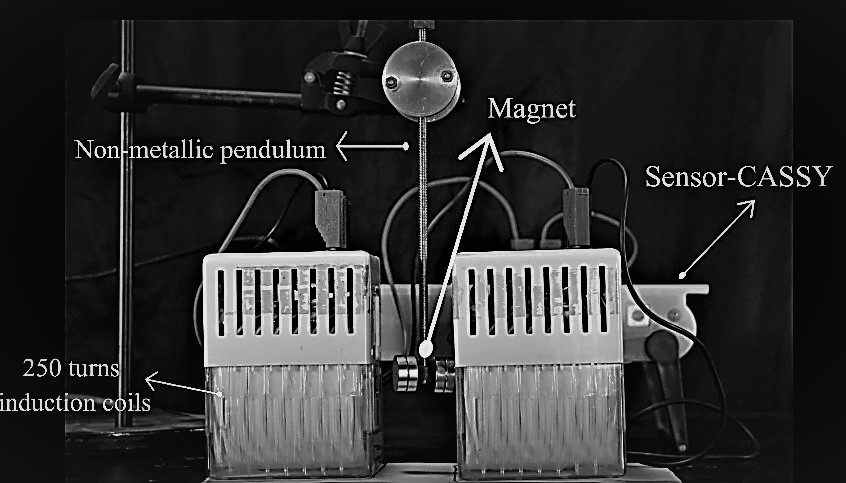
\includegraphics[width=10cm, height=7cm]{figures/fig4.jpeg} \\
 A Non-metallic pendulum is suspended with two magnets, two 250 turns induction coils and a CASSY Sensor is attatched as above to record the motion and amplitude of the oscillator that is damped in air.A rule was used to take the measurement of the length of the pendulum. 


\section{Method / Procedure}

The length of the pendulum is measured using the metre Rule. The two coils were placed close to the magnets and the pendulum was oscillated. CASSY was used to record the data for 50 seconds to view damping. The same process is repeated 3 times for different pendulum lengths. \\
Data of the length of pendulum and its amplitude with time was collected to analyse damping.

\section{Data}

Since the length of the pendulum was only measured once , it does not have type A uncertainty. The type B uncertainty associated is 0.0002m.

\begin{figure}[h!]
    \centering
    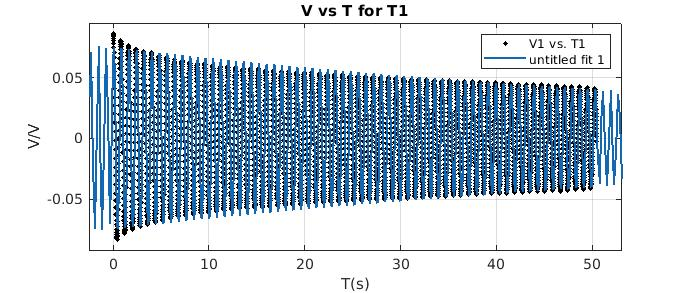
\includegraphics[width=\textwidth]{figures/L1.jpg}
    \caption{Graph of V vs T}
    \label{fig:yx}
\end{figure}
$$ x(t) = 0.07449^{-0.01244t} \times cos(7.873t -0.08103) $$
\newpage
\begin{figure}[h!]
    \centering
    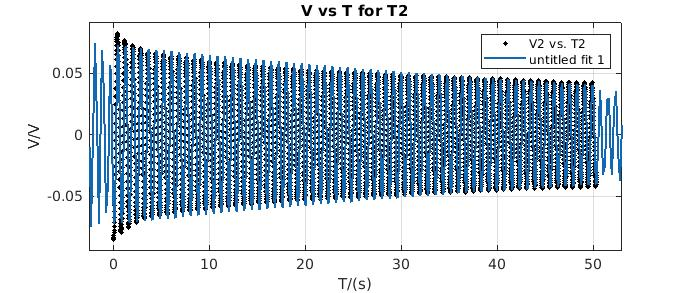
\includegraphics[width=\textwidth]{figures/L2.jpg}
    \caption{Graph of V vs T}
    \label{fig:yx}
\end{figure}
%m_v2 = -0.07236*exp(-0.01184.*T2).*cos(7.882.*T2-0.42);
$$ x(t) = -0.07236^{-0.01184t} \times cos(7.882t -0.42) $$
\newpage
\begin{figure}[h!]
    \centering
    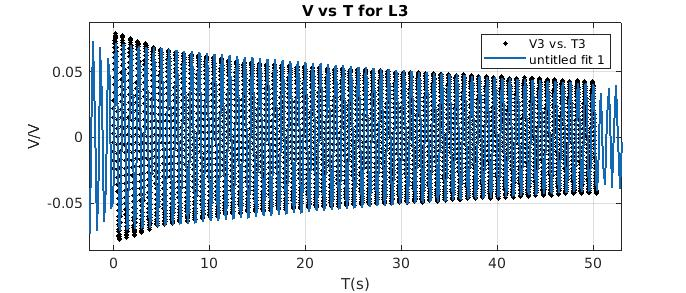
\includegraphics[width=\textwidth]{figures/L3.jpg}
    \caption{Graph of V vs T}
    \label{fig:yx}
\end{figure}
%m_v3 = 0.07135*exp(-0.01141.*T3).*cos(7.965.*T3-1.922);
$$ x(t) = 0.07135^{-0.01141t} \times cos(7.965t - 1.922)$$
\newpage\begin{figure}[h!]
    \centering
    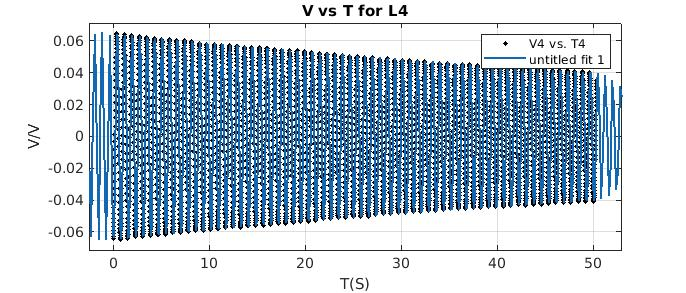
\includegraphics[width=\textwidth]{figures/L4.jpg}
    \caption{Graph of V vs T}
    \label{fig:yx}
\end{figure}
%m_v4 = -0.06439*exp(-0.009528.*T4).*cos(8.031*T4-0.1526);
$$ x(t) = -0.06439^{-0.009528t} \times cos(8.031t - 0.1526)$$
\newpage
\begin{figure}[h!]
    \centering
    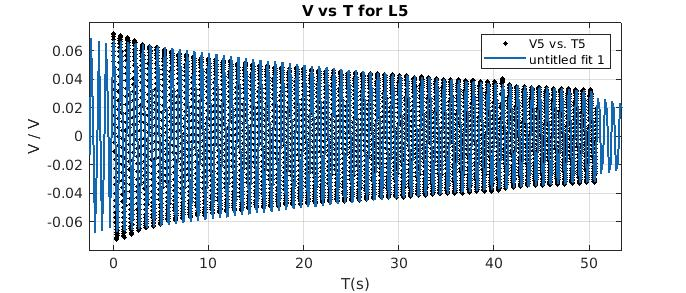
\includegraphics[width=\textwidth]{figures/L5.jpg}
    \caption{Graph of V vs T}
    \label{fig:yx}
\end{figure}
%m_v5 = 0.0673*exp(-0.01495.*T5).*cos(8.142.*T5 - 0.07685);
$$ x(t) = 0.0673^{-0.01495t} \times cos(8.142t - 0.07685)$$
\section{Data Analysis}

\begin{figure}[h!]
    \centering
    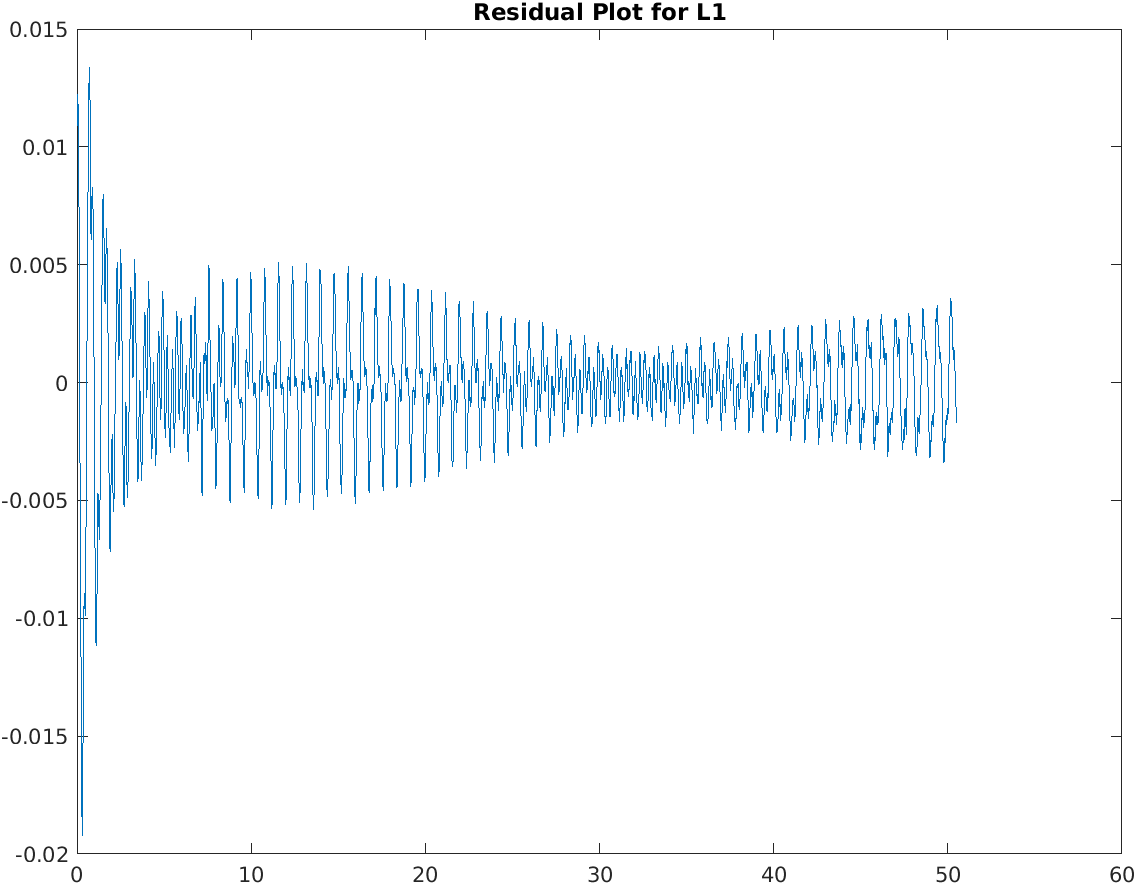
\includegraphics[width=\textwidth]{figures/L1_R.png}
    \caption{Residual Plot for L1}
    \label{fig:yx}
\end{figure}
\newpage
\begin{figure}[h!]
    \centering
    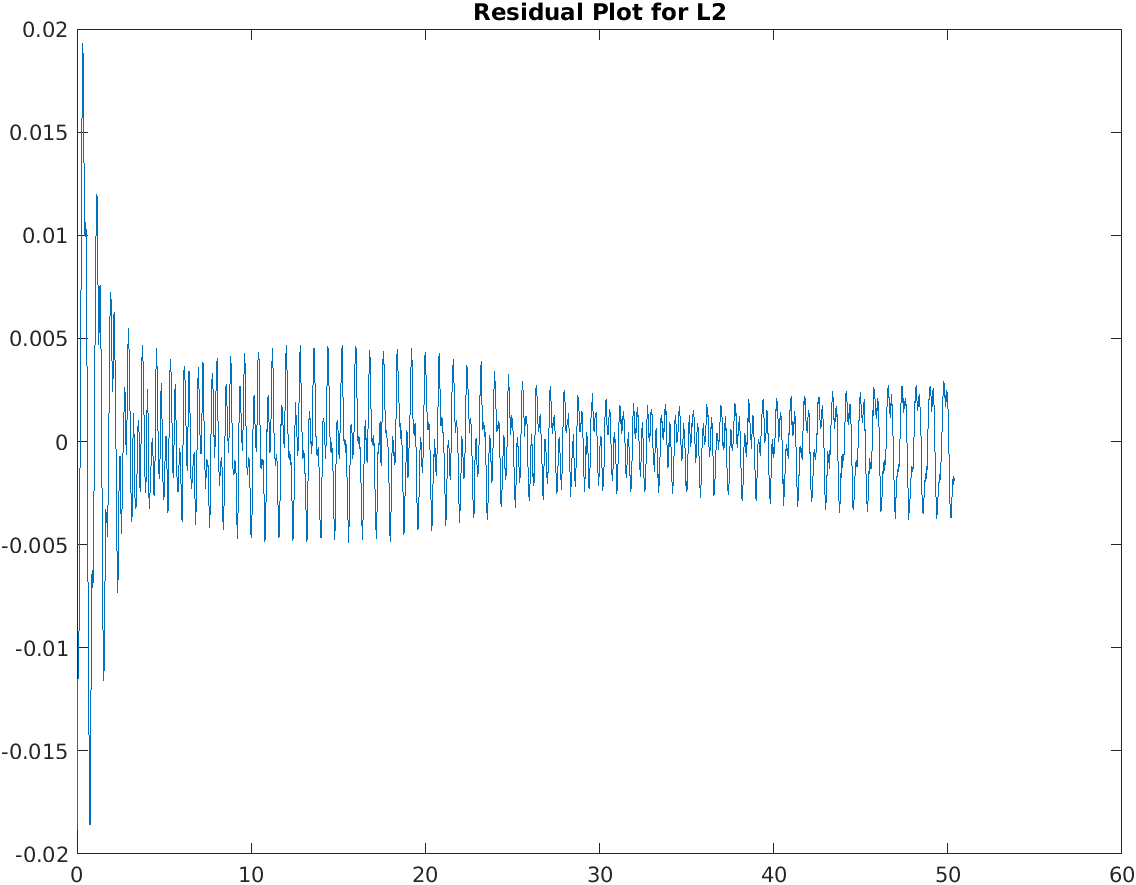
\includegraphics[width=\textwidth]{figures/L2_R.png}
    \caption{Residual Plot for L2}
    \label{fig:yx}
\end{figure}
\newpage
\begin{figure}[h!]
    \centering
    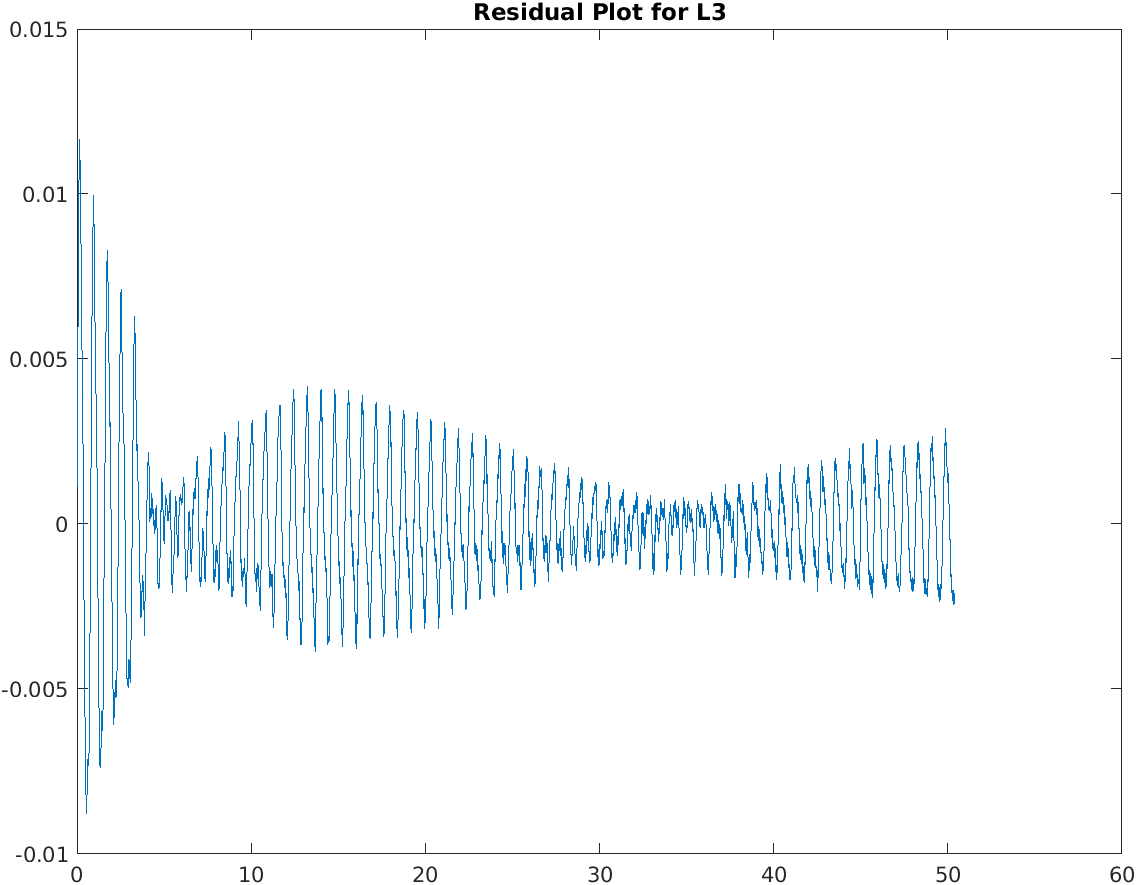
\includegraphics[width=\textwidth]{figures/L3_R.png}
    \caption{Residual Plot for L3}
    \label{fig:yx}
\end{figure}
\newpage
\begin{figure}[h!]
    \centering
    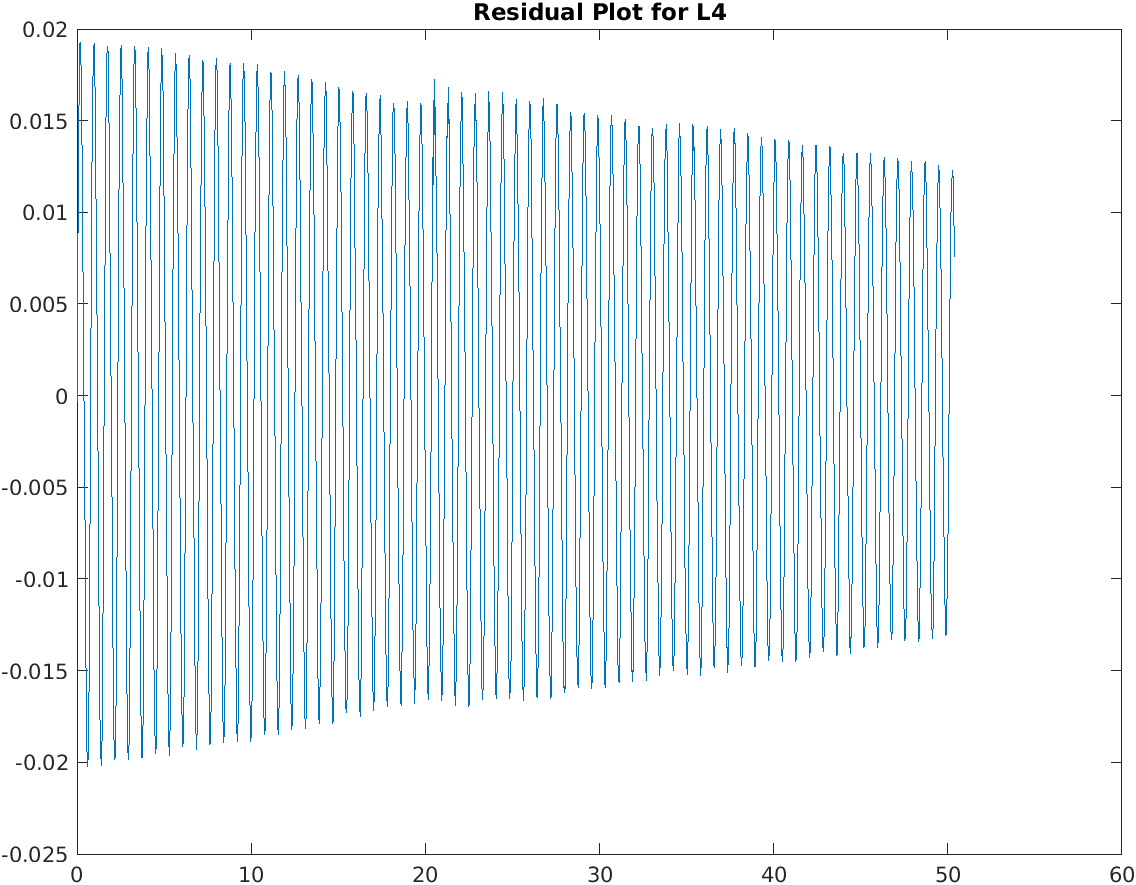
\includegraphics[width=\textwidth]{figures/L4_R.png}
    \caption{Residual Plot for L4}
    \label{fig:yx}
\end{figure}
\newpage
\begin{figure}[h!]
    \centering
    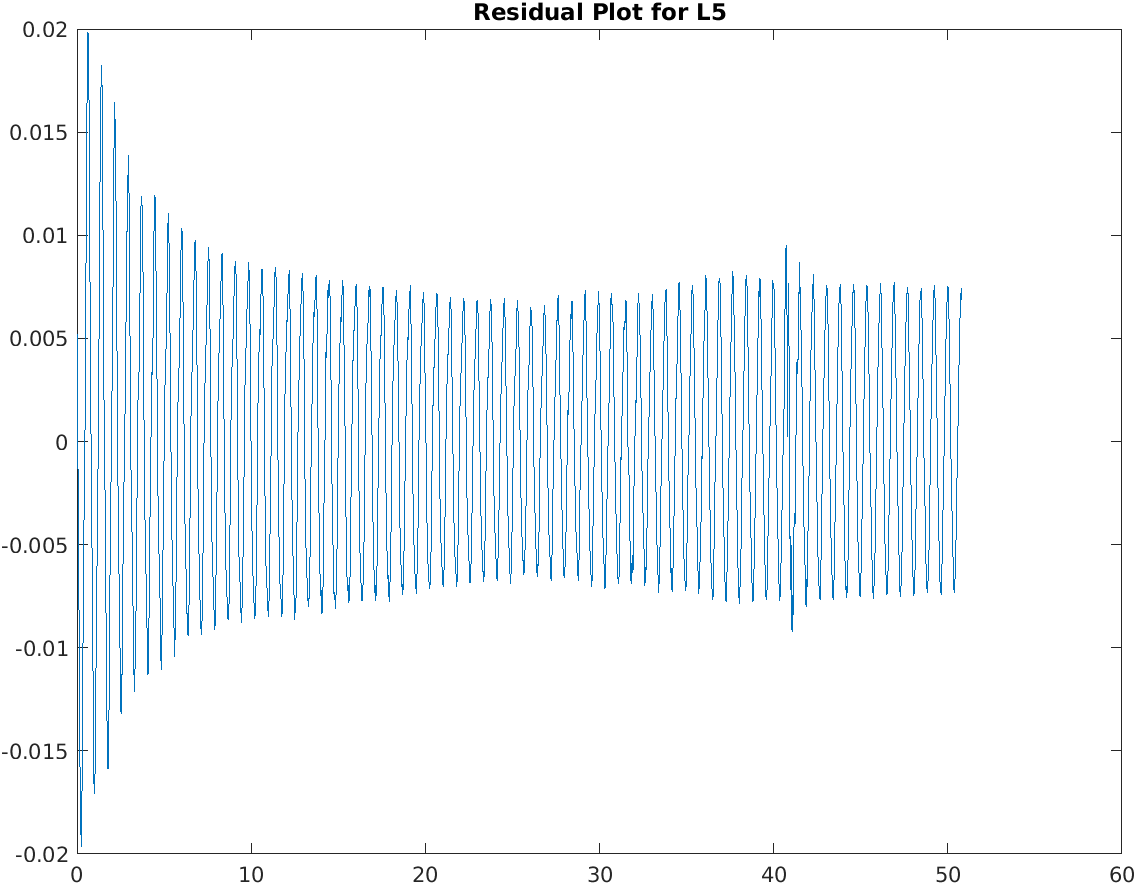
\includegraphics[width=\textwidth]{figures/L5_R.png}
    \caption{Residual Plot for L5}
    \label{fig:yx}
\end{figure}


\newpage
\begin{figure}[h!]
    \centering
    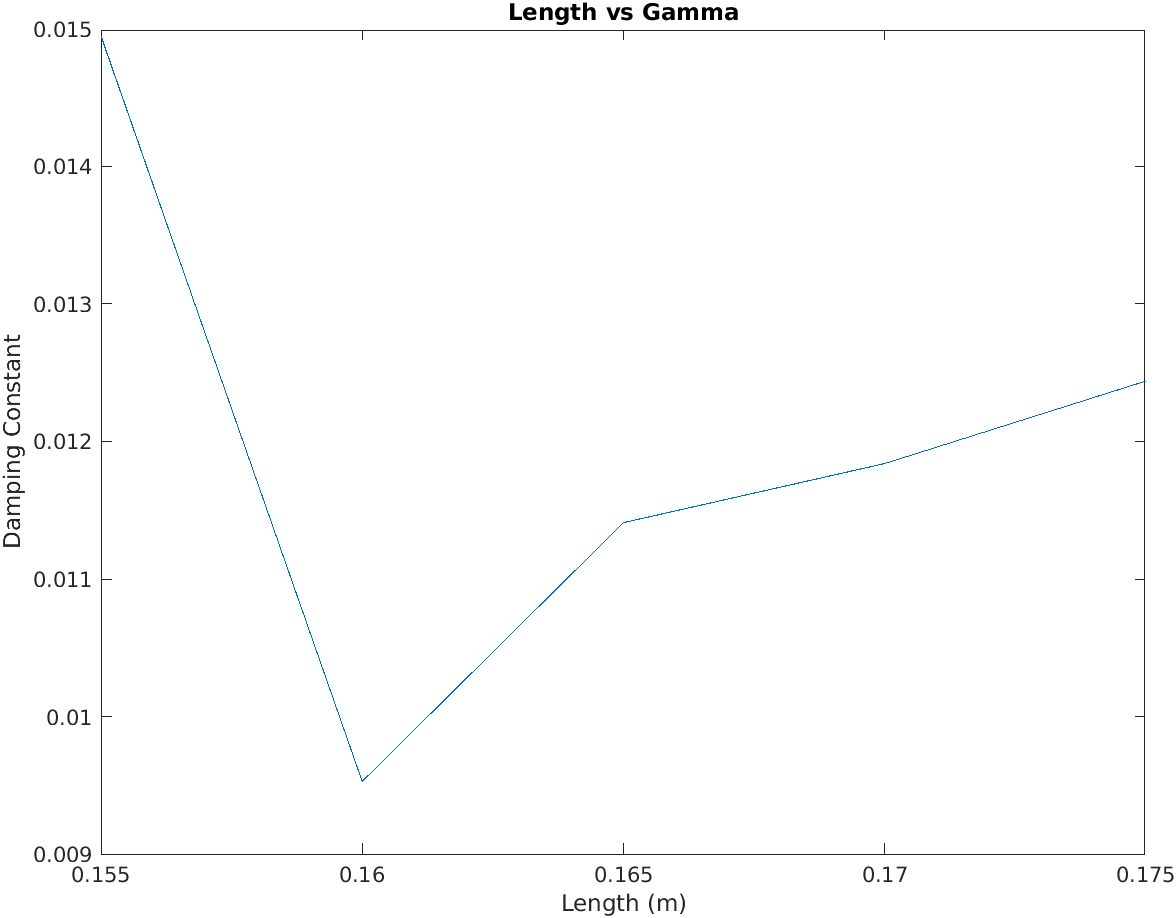
\includegraphics[width=\textwidth]{figures/L vs G.png}
    \caption{Graph of Length  vs Damping Constant}
    \label{fig:yx}
\end{figure}

\section{Discussion \& Conclusion}

The graph of the the damping constants vs length and the residual plots show have random pattern which indicate the presence of random errors. The experiment could have been improved by ensuring that there was no wind in the room while doing the experiment. 


\section{MATLAB Script}
\lstinputlisting{matlabCodes/Experiment3.m}



